\section*{Теория}

Явление отклонения от распространения света согласно законам геометрической оптики, называется \textit{дифракцией} в широком смысле слове. В узком смысле слова дифракцией называется явление огибания светом препятствия и проникновение в область геометрической тени.

\subsection*{Основная задача дифракции}

\begin{wrapfigure}{left}{0.38\textwidth}
	\centering
	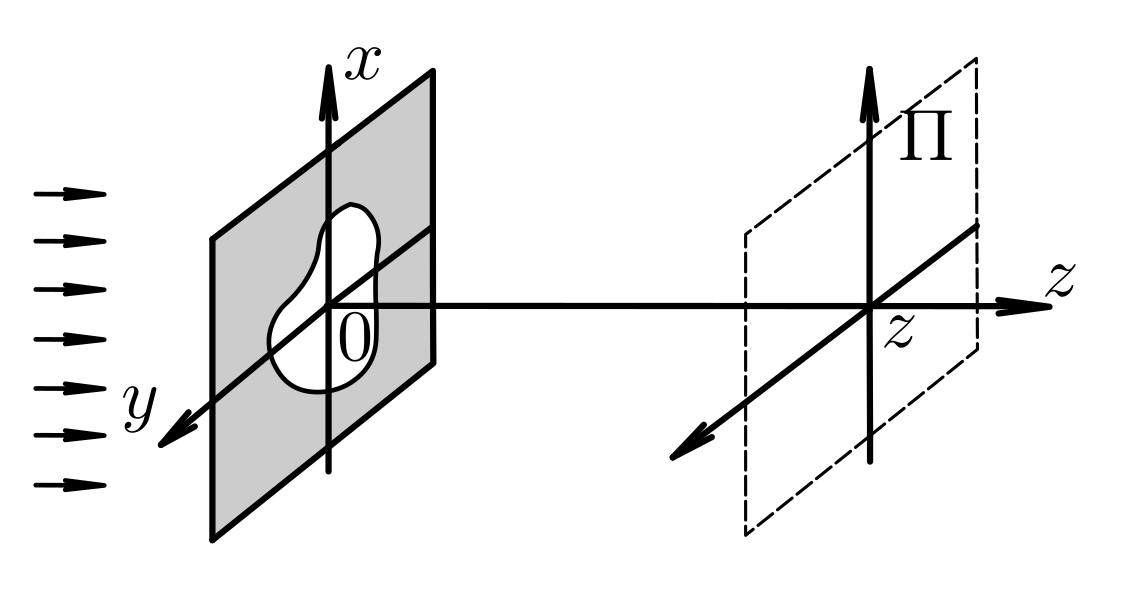
\includegraphics[width=0.38\textwidth]{../Изображения/Задача дифракции.png}
	\caption{Основная задача дифракции}
\end{wrapfigure}

При рассмотрении явления дифракции решается следующая основная задача.

Пусть в плоскости $z = 0$ находится экран с отверстием произвольной формы, и в полупространстве $z < 0$ находятся источники излучения. Пусть известно результирующее поле от источников $f_и(x, y, 0)$, которое они создают в плоскости $z = 0$ в отсутствии экрана. Тогда
\begin{enumerate}
	\item Зная оптические свойства материала, из которого изготовлен экран и геометрические размеры отверстия, необходимо найти распределение поля $f_0(x, y, 0)$ сразу после экрана, в плоскости $z = +0$.
		
	\item По распределению поля на границе экрана $f_0(x, y, 0)$ нужно найти значение поля в области пространства $z > 0$, в частности на исследуемой поверхности $П$, находящейся на расстоянии $z$ от экрана.
\end{enumerate}

Получить аналитическое выражение для электромагнитного поля на границе экрана $f_0(x, y, 0)$ часто не возможно. Во-первых, электромагнитная волна на поверхности экрана порождает переменные токи. Электромагнитное поле индуцированных токов необходимо учитывать при вычислении поля на границе экрана. Во-вторых, отверстие может иметь сложную геометрию. В-третьих, оптические свойства материала экрана могут быть не линейными.

Для упрощения решения основной задачи, применяется \textit{приближение Кирхгофа}. Предполагается, что поле в той части экрана, где есть отверстие равно результирующему полю источников $f_и(x, y, 0)$, если бы не было экрана. В области, затененной экраном поле источников считается равным 0. То есть в данном приближении пренебрегается взаимодействием экрана и электромагнитного поля. Данное приближение хорошо описывает реальные физические системы, если, во-первых, линейные размеры отверстия $b$ велики по сравнению с длиной волны $\lambda$: $b > \lambda$. Во-вторых, если плоскость наблюдения находится на расстоянии $z$ много большем длины волны: $z \gg \lambda$.

\subsection*{Принцип Гюйгенса-Френеля}

Согласно \textit{принципу Гюйгенса-Френеля}, каждая точка волнового фронта является источником вторичных сферических волн, а результирующее поле в исследуемой точке пространства --- результат интерференции вторичных волн.

\begin{wrapfigure}{left}{0.4\textwidth}
	\centering
	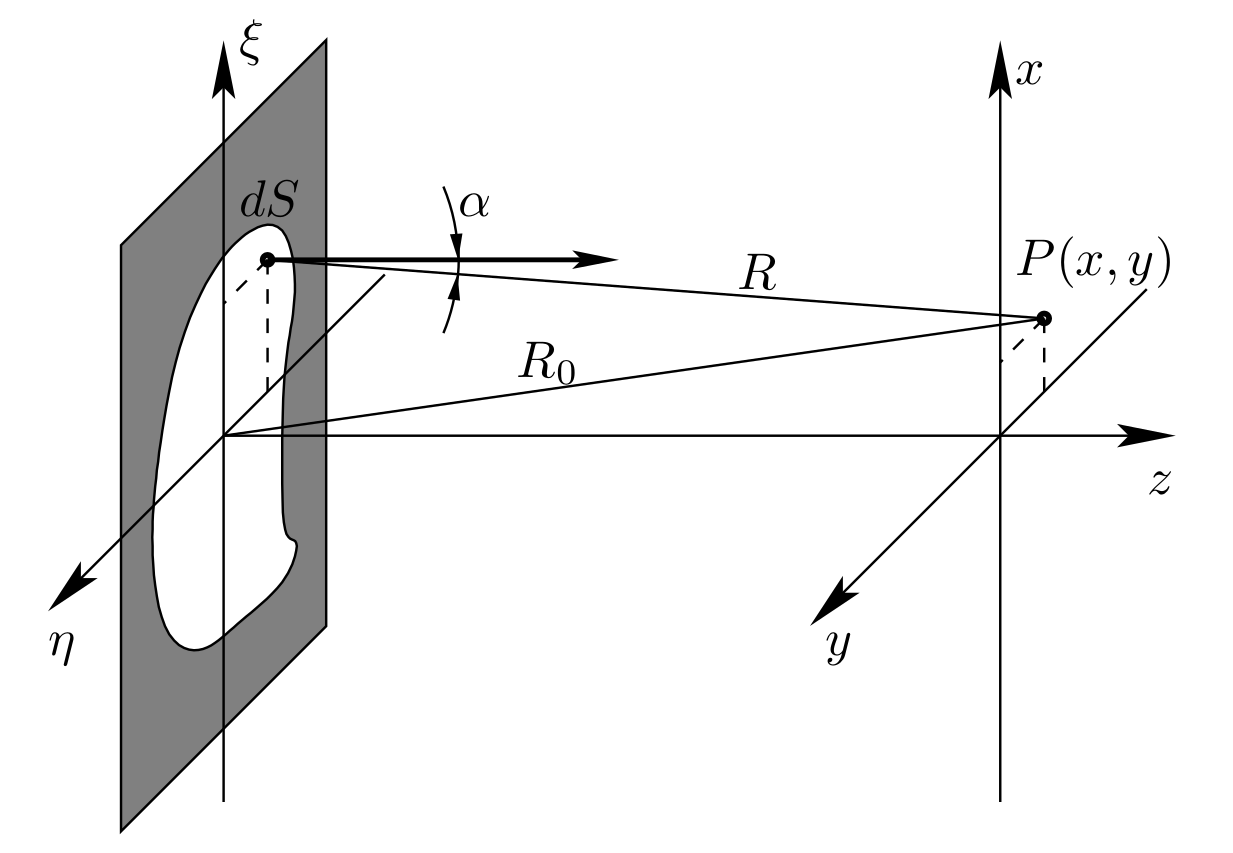
\includegraphics[width=0.38\textwidth]{../Изображения/Принцип Гюйгенса-Френеля.png}
	\caption{Принцип Гюйгенса-Френеля}
\end{wrapfigure}

Получим качественную оценку для поля в исследуемой точке пространства $P(x, y, z)$. Рассмотрим точку отверстия с координатами $(\xi, \eta)$. Она является источником вторичных сферических волн c амплитудой, пропорциональной амплитуде исходной волны. Фаза вторичной волны равна фазе исходной волны. В точке $P$ амплитуда сферической волны уменьшится в $R$ раз, фаза изменится на $e^{ikR}$. Предполагается, что амплитуда колебаний поля в исследуемой точке пропорциональна видимой площади $ds \cos \alpha$ элементарной площадки, создающей вторичные волны. Итого поле $d g(x, y)$, создаваемое в точке $P$, площадкой $ds$:
$$
dg(x, y) \sim f_0(\xi, \eta) \frac{e^{ikR}}{R} \cos \alpha d\xi d\eta
$$
Интегрируя по всей области отверстия получим выражение для результирующего поля $g(x, y)$ в точке $P$:
\begin{equation}
	g(x, y) = K_0 \iint\limits_S f_0(\xi, \eta) \frac{e^{ikR}}{R} \cos \alpha \, d\xi \, d\eta
	\label{theory:Huygens–Fresnel-prec}
\end{equation}
где коэффициент пропорциональности $K_0 = \frac{1}{i \lambda}$. Данное соотношение является количественной формулировкой принципа Гюйгенса-Френеля.

При использовании принципа Гюйгенса-Френеля используют следующие приближения. Во-первых, так как обычно рассматриваются параксиальные лучи, то расстояние $R$ от точек отверстия до всех точек исследуемой плоскости считается одинаковым и равным $R_0$:
$$
g(x, y) = \frac{1}{i \lambda R_0} \iint_S f_0(\xi, \eta) e^{ikR} \cos \alpha  \, d\xi \, d\eta
$$

Для оценки изменения фазы нужно использовать более точную оценку. Разложим расстояние $R$ по формуле Тейлора до второго порядка:
$$
R = \sqrt{z^2 + (x - \xi)^2 + (y - \eta)^2} \approx z + \frac{(x - \xi)^2}{2 z} + \frac{(y - \eta)^2}{2z}
$$
Предполагается, что члены разложения Тейлора более высокого вносят малую поправку в полученный результат. Такое приближение называется \textit{френелевским}. Итого значение поля в точке $P(x, y, z)$ вычисляется по формуле:
\begin{equation}
	g(x, y) = \frac{e^{ikz}}{i \lambda z} \iint\limits_S f_0(\xi, \eta) e^{i\frac{k}{2z}\left((x-\xi)^2 + (y - \eta)^2\right)} \, d\xi \, d\eta
	\label{theory:Huygens–Fresnel-approx}
\end{equation}

\subsection*{Дифракция Френеля на круглом отверстии}

\begin{wrapfigure}{left}{0.4\textwidth}
	\centering
	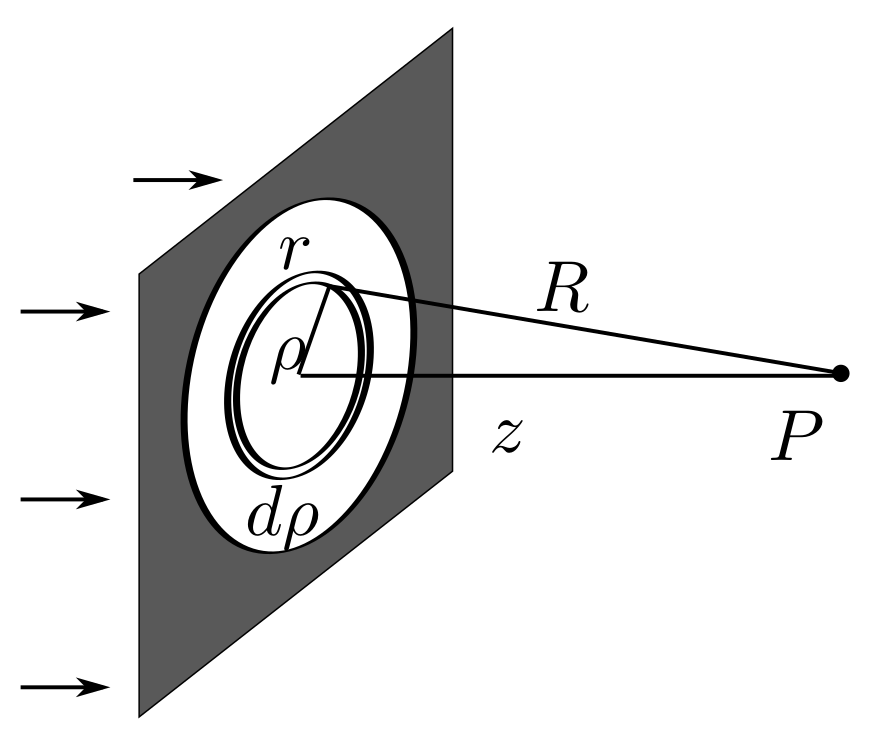
\includegraphics[width=0.38\textwidth]{../Изображения/Дифракция Френеля.png}
	\caption{Дифракция Френеля}
\end{wrapfigure}

Найдем распределение поля в точке $P(0, 0, z)$ от круглого отверстия радиуса $r$. Будем считать, что экран с отверстием освещается параллельным пучком световых волн с одинаковой амплитудой колебаний $A_0$. Тогда преобразуем формулу ($\ref{theory:Huygens–Fresnel-approx}$), перейдя к интегрированию по кольцам радиуса $\rho$, толщиной $d\rho$ и площадью $ds = 2 \pi \rho d \rho$:
$$
	g = A_0 \frac{e^{ikz}}{i \lambda z} \int \limits_0^r e^{i\frac{k}{2z} \rho^2} 2\pi \rho d \rho = A_0 e^{ikz} \left( 1 - e^{-ik\frac{k}{2z}r^2} \right)
$$
Интенсивность поля в точке $P$ вычисляется по формуле:
\begin{equation}
	I \propto <|g|^2> = 2I_0 \left(1 - \cos \left( \frac{k}{2z}r^2 \right)\right)
	\label{eq:Fresnels-intensity}
\end{equation}
где $I_0$ -- интенсивность исходной волны, усреднение производится за время много больше периода колебаний электромагнитной волны.

Проанализируем полученный результат. Точки $r_m = \sqrt{m \lambda z}, m = 1, 2, 3, \dots$ являются точками экстремума функции интенсивности. При нечётных $m$ наблюдается максимум $I_{max} = 4I_0$, при чётных $m$ -- минимум $I_{min} = 0$.

Полученное соотношение справедливо, когда $\frac{\cos \alpha}{R} \approx \frac{1}{R_0}$. С помощью \textit{метода векторных диаграмм} качественно учтем влияние множителя $\frac{\cos \alpha}{R}$ на результат.

Рассмотрим последовательность колец радиусом $\rho_n$, достаточно малой толщины $d \rho_n << 1$ и одинаковой площади $dS_n = dS_{n+1} = dS$. Тогда вклад от одного кольца в поле в точке $P$ обозначим в виде вектора $d \boldsymbol{A}$ на векторной диаграмме. Модуль этого вектора $dA = A_0 \frac{\cos \alpha}{\lambda R} dS$. Угол наклона вектора относительно горизонтали обозначим за $\varphi = \frac{k}{2z} \rho^2$. Угол между двумя соседними векторами $d \varphi = \frac{k}{z} \rho d \rho = \frac{1}{\lambda z} dS$ -- постоянная величина. 

\begin{wrapfigure}{left}{0.4\textwidth}
	\centering
	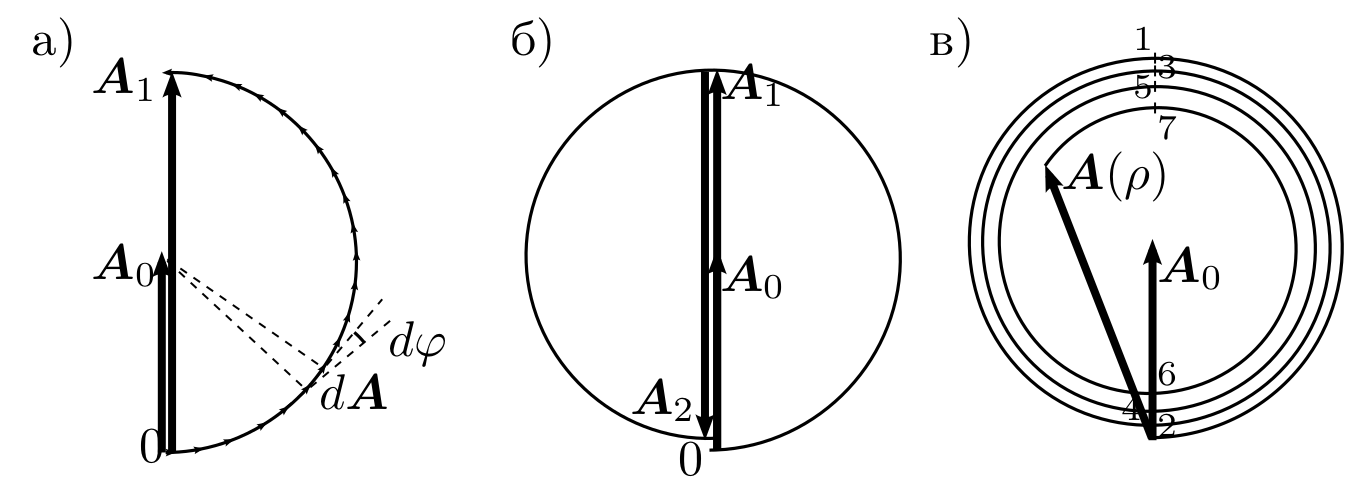
\includegraphics[width=0.38\textwidth]{../Изображения/Векторные диаграммы.png}
	\caption{Метод векторных диаграмм. Спираль Френеля.}
	\label{img:Fresnel-spiral}
\end{wrapfigure}

Векторы $d \boldsymbol{A}$, построенные последовательно друг за другом будут образовывать спираль, медленно скручивающуюся к центру (модуль вектора $dA$ убывает с увеличением радиуса кольца). Результирующее поле $\boldsymbol{A}(\rho)$ в точке $P$ равно сумме вкладов отдельных колец $d\boldsymbol{A}$ (рис. $\ref{img:Fresnel-spiral}$в).

Кольцо $r_{m - 1} < \rho < r_{m}$, где $r_m = \sqrt{m \lambda z}$ называется $m$-ой зоной Френеля. Не трудно показать, что результирующие колебания, создаваемые двумя последовательными зонами Френеля, сдвинуты по фазе на $\pi$. На векторной диаграмме зонам Френеля соответствуют полуокружности. На рисунке $\ref{img:Fresnel-spiral}$а изображена первая зона Френеля, результирующий вектор $A_1 = 2 A_0$. На рисунке $\ref{img:Fresnel-spiral}$б открыты две зоны Френеля и результирующее поле в точке $P$ мало, но не равно нулю.

Если открыто нечётное число зон Френеля, то наблюдается максимум амплитуды, если открыто чётное число зон Френеля, то -- минимум. При открытии большого числа зон Френеля вектор результирующих колебаний $A(\rho)$ медленно стремится к центру спирали и в пределе полностью открытого пространства равен по амплитуде колебаниям поля источников $A_0$.

\subsection*{Дифракция Френеля на узкой щели}

Рассмотрим бесконечно длинную узкую щель. Направим ось $\eta$ вдоль длинной стороны. Пусть вдоль оси $\xi$ края щели имеют координаты $b_1$ и $b_2$. Определим амплитуду колебаний света в точке $P(0, 0, z)$. Преобразуем двойной интеграл в формуле ($\ref{theory:Huygens–Fresnel-approx}$) к повторному:
$$
	g = \frac{e^{ikz}}{i \lambda z} \int \limits_{b_1}^{b_2} f_0(\xi, \eta) e^{i\frac{k}{2z}\xi^2} \, d\xi \int \limits_{-\infty}^{+\infty} e^{i\frac{k}{2z} \eta^2} \, d\eta 
$$
Интеграл по $\eta$ является интегралом Пуассона и равен константе:
$$
	\int \limits_{-\infty}^{+\infty} e^{i\frac{k}{2z} \eta^2} \, d\eta  = \sqrt{\pi}
$$
С учетом данного соотношения преобразуем формулу для вклада :
$$
	g = A_0 \int \limits_{b_1}^{b_2} f_0(\xi, \eta) e^{i\frac{k}{2z}\xi^2} \, d\xi
$$

Проанализируем полученное соотношение, используя метод векторных диаграмм. Разобьем щель на узкие бесконечно длинные полоски шириной $d \xi$. Каждая такая полоска вносит вклад в колебание поля в точке $P$ равный $d \boldsymbol{A}$. Модуль этого вектора равен $d A = A_0 \cdot d \xi$, угол наклона относительно горизонтали $\varphi = \frac{k}{2z} \xi^2$. Угол между соседними векторами $d \varphi = \frac{k}{z} \xi d\xi \neq const$. Полученная формула сильно похожа на формулу, полученную в случае дифракции Френеля на круглом отверстии. Для круглого отверстия $d \varphi = const$, так как кольца выбирались так, что их площадь была постоянной $d S = 2 \pi \rho d \rho = const$. Для узких бесконечно длинных полосок, в отличие от тонких колец, нельзя выбрать шаг $d \xi$ так, чтобы одновременно $dA = const$ и $d \varphi = const$.

\begin{wrapfigure}{left}{0.4\textwidth}
	\centering
	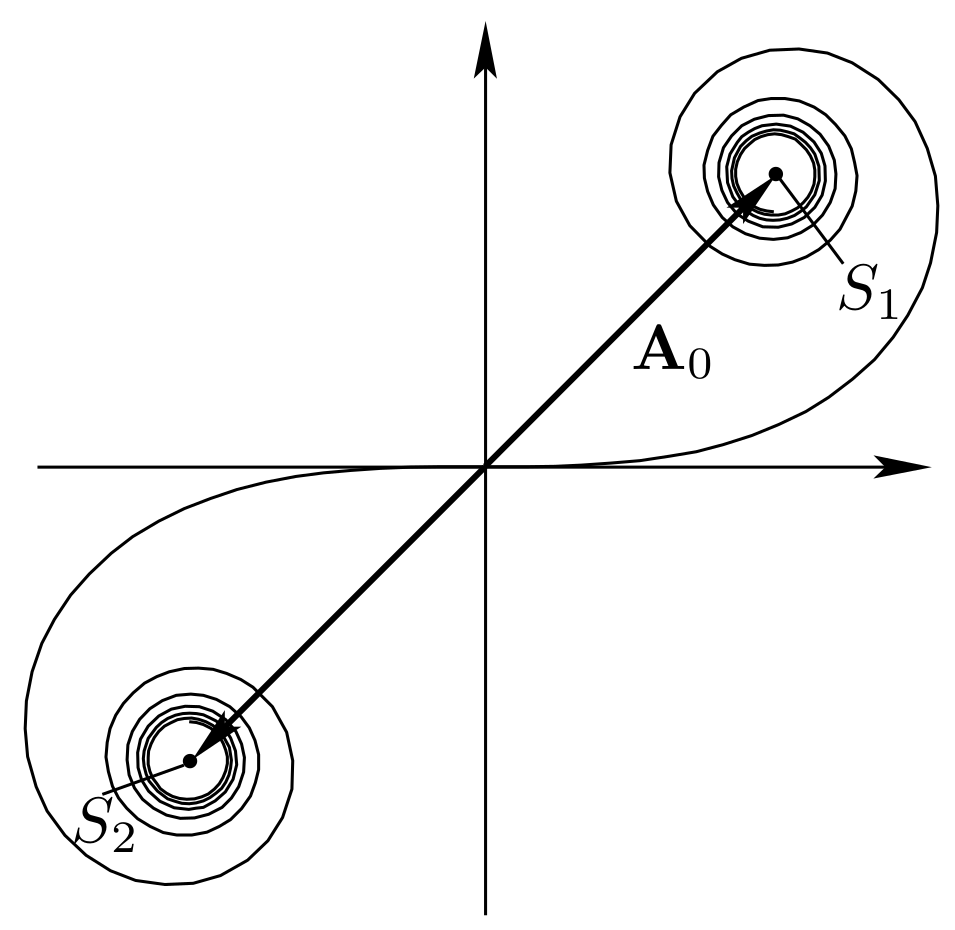
\includegraphics[width=0.38\textwidth]{../Изображения/Спираль Корню.png}
	\caption{Метод векторных диаграмм. Спираль Корню.}
	\label{img:Cornu-spiral}
\end{wrapfigure}

В результате сложения вкладов отдельных полосок конец вектора результирующей амплитуды колебаний будет описывать спираль Корню. Когда вектор $d \boldsymbol{A}$ повернётся относительно начального на $\pi$, то полосу $\xi \in [0; \pi]$ называют первой зоной Шустера. Полосу $\xi \in [\xi_{m-1}; \xi_m]$, где $\xi_m = \sqrt{m \lambda z}$ называют $m$-ой зоной Шустера.

Спираль Корню быстро скручивается к фокусам $S_1$ и $S_2$ при открытии большого числа зон Шустера. При открытии двух зон, амплитуда колебаний близка к максимальной. При открытии бесконечно большого числа зон Шустера, вектор результирующих колебаний соединяет фокусы спирали и по модулю равен $A_0$ - амплитуде колебаний поля источников.

\subsection*{Условия, определяющие тип дифракции}

Пусть размер характерный размер отверстия равен $b$. Тогда всего будет открыто $m$ зон Френеля (Шустера):
$$
m = \frac{b^2}{\lambda z} = \frac{1}{p^2}
$$
где $p$ -- волновой параметр, определяющий тип дифракции.

Если $p \ll 1$ ($m \gg 1$), то открыто почти всё пространство и свойства распространения света описываются геометрической оптикой. Если $p \sim 1$ ($m \sim 1$), то наблюдается дифракция Френеля. Если $p \gg 1$ ($m \ll 1$), то наблюдается дифракция Фраунгофера.

\subsection*{Дифракция Фраунгофера}

Рассмотрим дифракцию на отверстии с максимальным размером $b$. То есть $\xi^2 + \eta^2 \le b^2$. Определим амплитуду колебаний в точке $P(x, y, z)$. Расстояние от точки $P$ до площадки $dS$ - источника вторичных волн равно
$$
R = \sqrt{z^2 + (x - \xi)^2 + (y - \eta)^2} = \sqrt{R_0 - (2x \xi + 2 y \eta) + (\xi^2 + \eta^2)}
$$
где $R_0 = \sqrt{x^2 + y^2 + z^2}$. Рассмотрим параксиальное приближение, когда расстояние до наблюдаемой точки много больше размеров отверстия, тогда
$$
R \approx R_0 - \frac{x\xi + y \eta}{R_0} + \frac{\xi^2 + \eta^2}{2R_0} \approx  R_0 - \frac{x\xi}{R_0} - \frac{y \eta}{R_0}
$$
здесь применяется приближение $\xi^2 + \eta^2 \le b \ll R_0$.

Принцип Гюйгенса-Френеля для дифракции Фраунгофера:
$$
g(x, y) = \frac{e^{i kR_0}}{i \lambda R_0} \iint \limits_S f_0(\xi, \eta) e^{-i \left(\frac{kx}{R_0}\xi + \frac{ky}{R_0}\eta\right)} \, d\xi \, d\eta
$$

Введем переменные $u = \frac{kx}{R_0}$, $v = \frac{ky}{R_0}$, тогда формула для колебаний поля в точке плоскости наблюдения $P(u, v)$ есть двумерное преобразование Фурье:
$$
g(u, v) = \frac{e^{i kR_0}}{i \lambda R_0} \iint \limits_S f_0(\xi, \eta) e^{-i (u \xi + v \eta )} \, d\xi \, d\eta
$$

\begin{wrapfigure}{left}{0.4\textwidth}
	\centering
	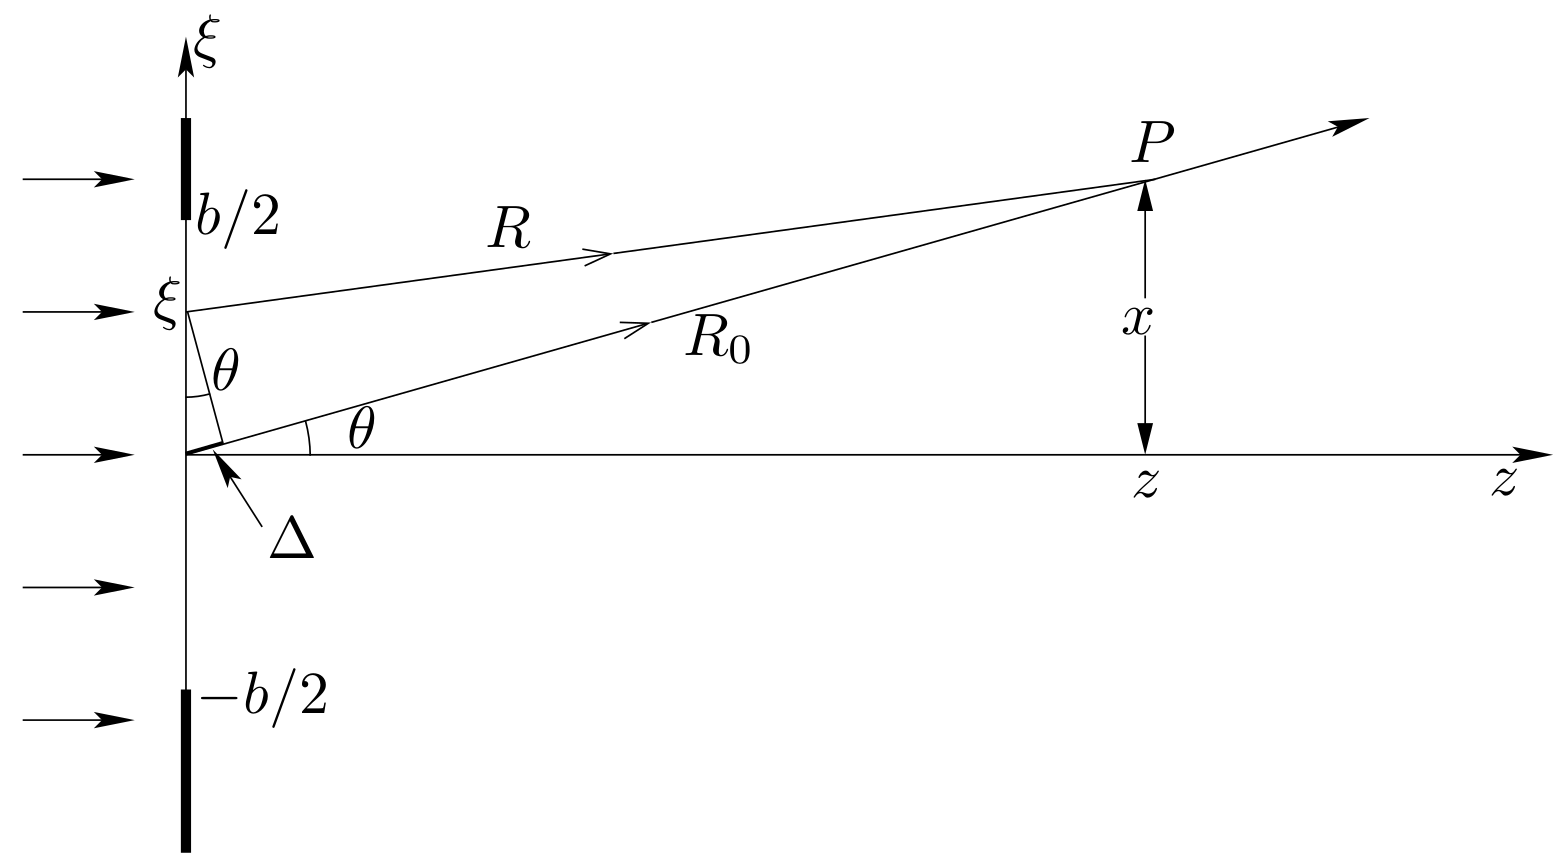
\includegraphics[width=0.38\textwidth]{../Изображения/Дифракция Фраунгофера в одномерном случае.png}
	\caption{Дифракция Фраунгофера в квазиодномерном случае}
	\label{img:Fraunhofer-quasi-one-dimensional}
\end{wrapfigure}

Рассмотрим квазиодномерный случай, когда $f_0(\xi, \eta) = f_0(\xi)$. Тогда амплитуда поля в наблюдаемой точке определяется выражением:
$$
g(u) = A_0 \int \limits_{-\infty}^{+\infty} f_0(\xi) e^{-i u \xi} \, d\xi
$$

Определим разность хода лучей из двух точек экрана с расстоянием $\xi$ между ними. В приближении параксиальной оптики, можно считать лучи параллельными, и разность хода определяется выражением $\Delta = \xi \sin \theta$. Тогда разность фаз $\Delta \varphi = k \xi \sin \theta = \frac{k x}{R_0} = u$. Тогда выражение, определяющее амплитуду колебаний в наблюдаемой точке, преобразуется к виду:
$$
g(u) = A_0 \int \limits_{-\infty}^{+\infty} f_0(\xi) e^{-i k \sin \theta \xi} \, d\xi
$$
Полученное соотношение аналогично преобразованию Фурье временной зависимости $f_0(t)$ в спектр:
$$
C(\omega) = \int f_0(t) e^{-i \omega t} dt
$$
Поэтому $u = k \sin \theta$ называют пространственной частотой по аналогии с временной частотой $\omega$.

В параксиальном случае положение точки полностью определяется углом $\theta$, поэтому значение амплитуды колебаний поля в наблюдаемой точке не изменится, если точку перемещать вдоль луча, соединяющего её с отверстием. Данное свойство используется для наблюдения дифракции Фраунгофера. В лабораторных условиях не возможно удалить наблюдаемую плоскость на достаточно большое расстояние от отверстия. Поэтому между наблюдаемым экраном и отверстием ставится собирающая линза. Параллельные лучи, падающие на собирающую линзу под углом $\theta$ она фокусирует в фокальной плоскости на расстоянии $f \sin \theta$ от главного фокуса. Поэтому наблюдаемое распределение интенсивности после прохождения света линзы не изменится (изменится лишь  масштаб наблюдаемого распределения).

\begin{wrapfigure}{left}{0.6\textwidth}
	\centering
	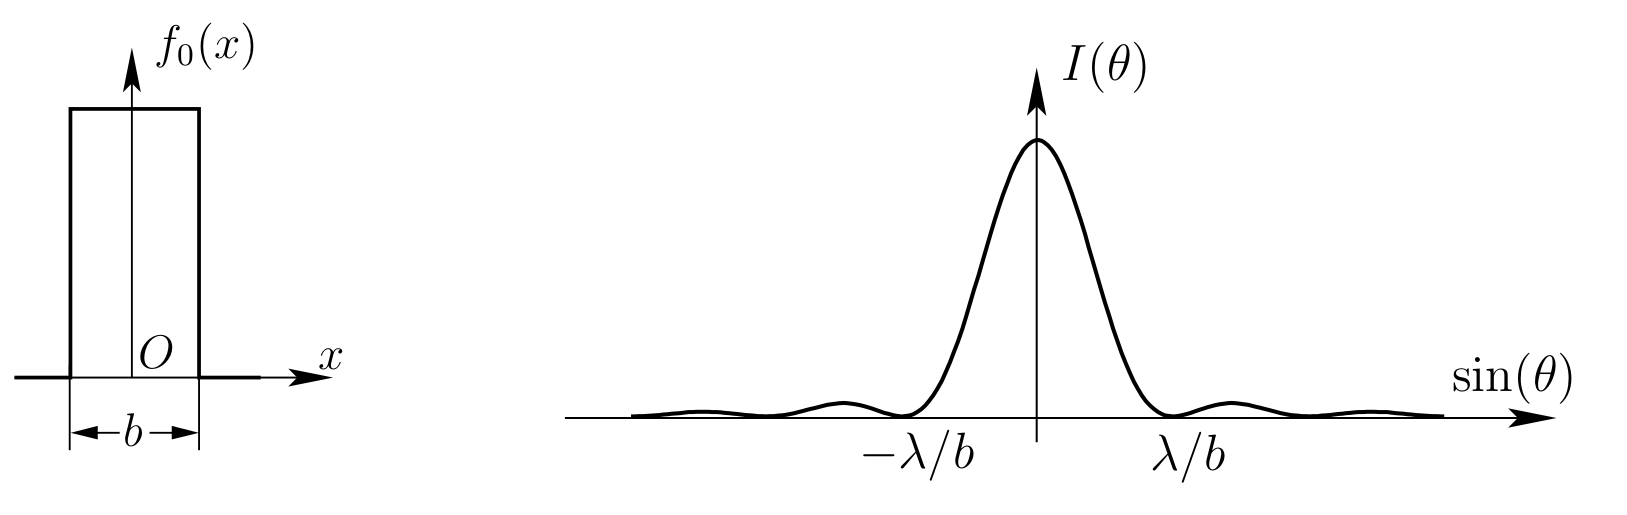
\includegraphics[width=0.58\textwidth]{../Изображения/Дифракция Фраунгофера на щели.png}
	\caption{Зависимость $f_0(x)$ (слева) и распределение интенсивности (справа) при дифракции на щели}
	\label{img:Fraunhofer-diffraction_slite}
\end{wrapfigure}

Рассмотрим дифракцию Фраунгофера на щели. Пусть щель освещается параллельным пучком света с амплитудой колебаний $f_0$. Распределение амплитуды колебаний $f_0(x)$ описывается прямоугольным импульсом (рис. $\ref{img:Fraunhofer-diffraction_slite}$).

Для определения амплитуды колебаний поля в наблюдаемой плоскости применим преобразование Фурье:
$$
g(\theta) = A_0 \frac{\sin \left( \frac{kb}{2} \sin \theta \right)}{\frac{kb}{2} \sin \theta}
$$
Распределение интенсивности в зависимости от направления $\theta$ изображено на рисунке $\ref{img:Fraunhofer-diffraction_slite}$ справа. По этой зависимости видно, что в угловом конусе $|\sin \theta| \le \frac{\lambda}{b}$ сосредоточена большая часть потока энергии. Этот угловой конус называется \textit{главным максимумом}.